\documentclass[8pt]{beamer}

\usepackage[utf8]{inputenc}
\usefonttheme{structuresmallcapsserif}
\usetheme{Goettingen}

\title{Online Social Network Analysis: A Survey of Research Applications in Computer Science}
\subtitle{Social Network Analysis Mid-Term Presentation}
\author{Presented by {\newline}Sitdhibong Laokok {\newline}63199130350}
\date{2021}

\newcommand{\comment}[1]{}

\AtBeginSection[]
{
  \begin{frame}<beamer>
    \frametitle{Outline}
    \tableofcontents[currentsection]
  \end{frame}
}

\begin{document}


  \frame{\titlepage}
  
  \begin{frame}
  	\frametitle{Outline}
  	\tableofcontents
  \end{frame}

  \section{Introduction}
  \begin{frame}
  	\frametitle{Publication Information}
  	\begin{columns}
  		\column{0.5\textwidth}
  			\begin{itemize}
  				\item[--] \textbf{Online Social Network Analysis: A Survey of Research Applications in Computer Science}
  				\item[--] David Burth Kurka, Alan Godoy, and Fernando J. Von Zuben
  				\item[--] 2016
  			\end{itemize}
  		
  		\column{0.5\textwidth}
  		\begin{figure}
  			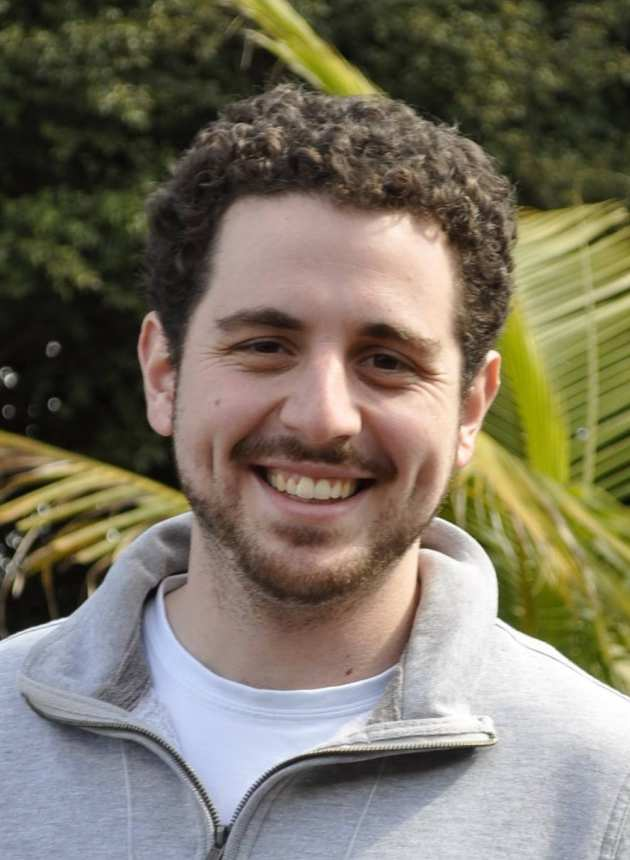
\includegraphics[scale=0.2]{asset/portrait.jpg}
  		\end{figure}
  	\end{columns}
  \end{frame}
  
  \begin{frame}
  	\frametitle{Social Networks}
  	\begin{figure}
  		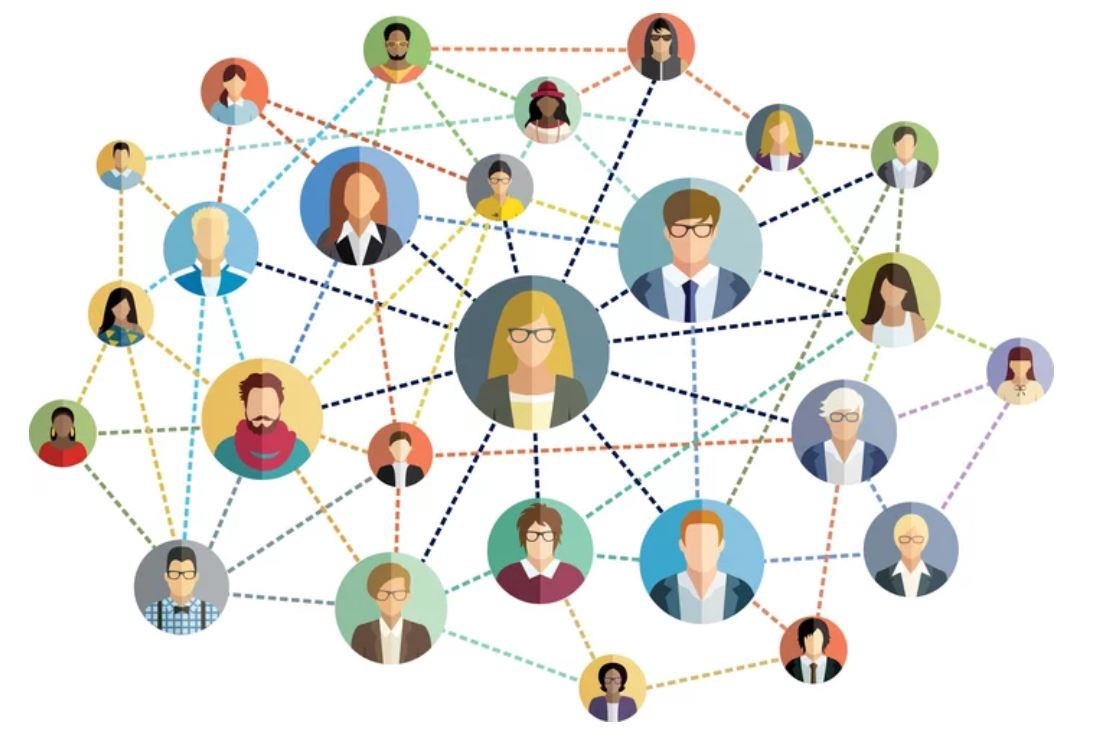
\includegraphics[scale=0.25]{asset/social-network.jpeg}
  	\end{figure}
  \end{frame}
  
  \begin{frame}
  	\frametitle{Online Social Networks}
  	
  	\vfill
  	
  	\begin{quotation}
  		The Internet is used for development for online social networks (OSNs) -- an adoptation of social organization to the "virtual world"
  	\end{quotation}
  	
  	\vfill
  	
  	\begin{figure}
  		\begin{minipage}{0.25\textwidth}
  			
\includegraphics[scale=0.08]{asset/google-plus-logo.jpg}
  		\end{minipage}
  		\begin{minipage}{0.25\textwidth}
  			
\includegraphics[scale=0.2]{asset/twitter-logo.eps}
  		\end{minipage}
  		\begin{minipage}{0.25\textwidth}
  			
\includegraphics[scale=0.035]{asset/facebook-logo.eps}
  		\end{minipage}
  	\end{figure}
  \end{frame}

  \section{Online Social Networks as Object of Study}

  \begin{frame}{Why should anyone research OSNs?}
    \begin{itemize}
      \item<1->[] \textbf{Data availability}:
      \item<2->[] \textbf{Multiple authorship}:
      \item<3->[] \textbf{Agent Interaction}:
      \item<4->[] \textbf{Temporal dynamics}:
      \item<5->[] \textbf{Instantaneity}:
      \item<6->[] \textbf{Ubiquity}:
    \end{itemize}
    
    \begin{figure}
    	\includegraphics<1>[scale=0.2]{asset/database.png}
    	\includegraphics<2>[scale=0.2]{asset/conversation.png}
    	\includegraphics<3>[scale=0.2]{asset/call-center-agent.png}
    	\includegraphics<4>[scale=0.2]{asset/exchange-rate.png}
    	\includegraphics<5>[scale=0.2]{asset/trending-topic.png}
    	\includegraphics<6>[scale=0.2]{asset/network.png}
    \end{figure}
    
  \end{frame}

  \begin{frame}{Which networks are explored?}
  
  	\vfill
  	\begin{itemize}
      \item<1->[] \textbf{Twitter}: Text Analysis
      \item<2->[] \textbf{Facebook}: Relationship, Networking
      \item<3->[] \textbf{YouTube}: Recommendation
      \item<4->[] \textbf{Flickr}: Image Processing
    \end{itemize}
  	
  	\vfill
  	\center
  	\begin{figure}
  		\begin{minipage}{0.2\textwidth}
  			\includegraphics<1->[scale=0.2]{asset/twitter-logo.eps}
  		\end{minipage}
  		\begin{minipage}{0.2\textwidth}
  			\includegraphics<2->[scale=0.040]{asset/facebook-logo.eps}
  		\end{minipage}
  		\begin{minipage}{0.2\textwidth}
  			\includegraphics<3->[scale=0.3]{asset/youtube.png}
  		\end{minipage}
  		\begin{minipage}{0.2\textwidth}
  			\includegraphics<4->[scale=0.04]{asset/flickr.png}
  		\end{minipage}
  	\end{figure}
  \end{frame}

  \begin{frame}{Computational tools}
	\vfill    
    \begin{itemize}
      \item Graph database: AllegroGraph, Neo4j
      \item Graph drawing software: Graphviz, Tulip
      \item Visualization: Cytoscape
      \item Analysis: igraph, NetworkX, NetworkKit
    \end{itemize}
    
    \vfill
  	\begin{figure}
  		\includegraphics<1>[scale=0.13]{asset/tools-neo4j.png}
  		\includegraphics<2>[scale=0.25]{asset/tools-graphviz.png}
  		\includegraphics<3>[scale=0.25]{asset/tools-cytoscape.png}
  		\includegraphics<4>[scale=0.5]{asset/tools-networkx.png}
  	\end{figure}
    
  \end{frame}
  
  \begin{frame}{Gephi - The Open Graph Viz Platform}
  	\begin{figure}
  		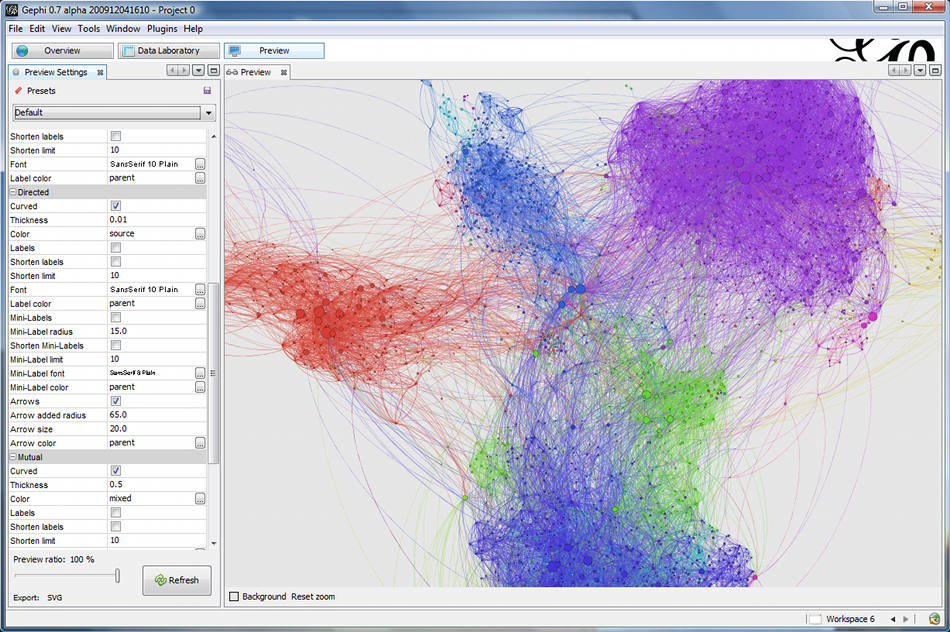
\includegraphics[scale=0.25]{asset/tools-gephi.png}
  		\caption{Gephi}
  	\end{figure}
  \end{frame}

  \section{Categories of Study}
  \begin{frame}{Categories of study on Online Social Networks}
    \begin{figure}
    	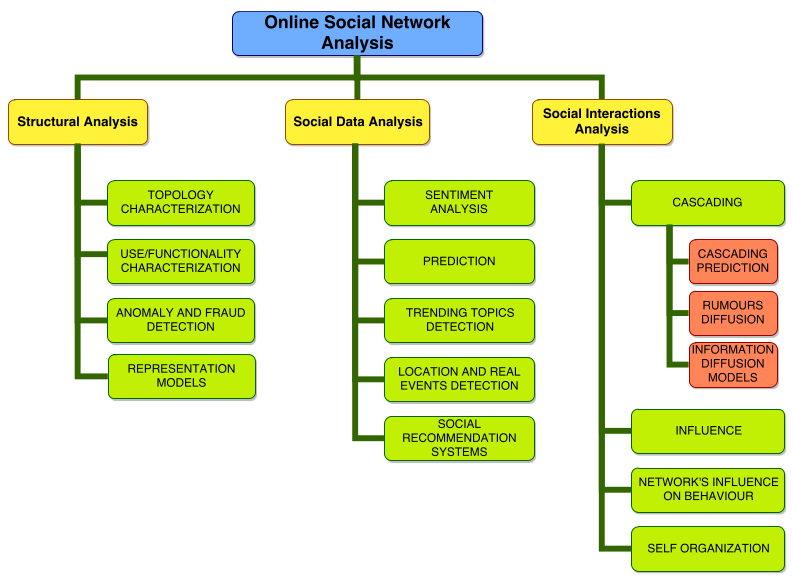
\includegraphics[scale=0.35]{asset/overview.png}
    \end{figure}
  \end{frame}
  
  \begin{frame}{Categories}
    \begin{itemize}
      \item \textbf{Structural analysis}: Simply knowing whate are those services and why so many people were being attracted to theme.
      \item \textbf{Social data analysis}: What OSNs produce.
      \item \textbf{Social interaction analysis}: How user interact on the network ad have isights o aspects of human behavior. This category discoveries relate to other fields of research, such as Psychology, Sociology and event Biology.
    \end{itemize}
  \end{frame}

  \section{Structural Analysis}
  \begin{frame}{Topology characterization}
  	\vfill
    \begin{itemize}
      \item \textbf{What the network structure reveals?}: How similar OSNs with real studied networks. This topics verified the presence of power-law degree distribution and small-world property.
      \item \textbf{Many network in one network}: OSN may embed more than one netowork structure. 
    \end{itemize}
    
    \vfill
    \begin{figure}
  		\includegraphics<1>[scale=0.3]{asset/watts-small-world.png}
  		\includegraphics<2>[scale=0.1]{asset/reliants_keyconcepts-03.png}
  		\includegraphics<3>[scale=0.3]{asset/six-degree-of-separation.png}
  	\end{figure}
    
  \end{frame}

  \begin{frame}{Use and functionality characterization}
    \begin{itemize}
      \item \textbf{Network formation}: User's interesting by geolocation distribution
      
      \item \textbf{User profiles}: To classify user characteristic by their behavior, such as \textit{Broadcasters} -- Celebrities, \textit{Acquaintances} -- Casual users, and \textit{Miscreants} -- Spammer, stalkers
      
      \item \textbf{Conversation}: To finding patterns and particularities that enabled the creation of a simple mathematical model capable of describing the dynamics of the conversations.
      
      \item \textbf{Network deterioration}: The impact of "cascades of users leaving" on the networks resilience was deeply studied, and a metric.
      
    \end{itemize}
  \end{frame}

  \begin{frame}{Anomaly and fraud detection}
    \begin{itemize}
      \item \textbf{Anomaly and fraud}: Structure can reveal the presence of anomalies, indicating that users might be acting in suspicious ways.
      
      \item \textbf{Spamming behavior}: Identified users acting as spammers considered the network's structural properties and also use the textual content of messages.
    \end{itemize}
  \end{frame}

  \begin{frame}{Representation models}
    \begin{itemize}
      \item \textbf{Structure models}: Singletons (users without connections), Isolated communities (generally around a popular user) and a Giant component (users connected to many users)
      
      \item \textbf{Spatio-temporal models}: To represent transformation processes taking place in a network.
    \end{itemize}
  \end{frame}

  \section{Social Data Analysis}
  \begin{frame}{Sentiment analysis}
 	\vfill
    \begin{itemize}
      \item<1-> \textbf{Taking advantage of corpora particularities}: Short message is adventage of sentiment classification, such as Tweet in Twitter. Text processing techniques were proposed to extract and reduce features and an algorithm was build reaching over 80\% of accuracy in classification. 
      
      \item<2-> \textbf{Applications}
    \end{itemize}
    
    \vfill
    \begin{figure}
  		\includegraphics<1>[scale=0.4]{asset/sentiment-analysis.png}
  		\includegraphics<2>[scale=0.2]{asset/sentimental-s-sence.png.png}
  		\includegraphics<3>[scale=0.2]{asset/sentimental-emoji.png}
  		
  		%\caption{
  		%	\only<1>{Sentiment Analysis} \\
  		%	\only<2>{S-Sense: http://www.ssense.in.th/} \\
  		%	\only<3>{AI for Thai: https://aiforthai.in.th/service_sa.php}
  		%}
  	\end{figure}
  	
  \end{frame}

  \begin{frame}{Prediction}
  	\vfill
  	\begin{itemize}
  		\item[--] \textbf{Elections}
  		\item[--] \textbf{Box-office revenue}
  		\item[--] \textbf{Book sales prediction}
  		\item[--] \textbf{Disease spread}
  		\item[--] \textbf{Stock market prediction for sentiment analysis}
  	\end{itemize}
  	
  	\vfill
  	\begin{figure}
  		\includegraphics<1>[scale=0.05]{asset/trump-election.jpg}
  		\includegraphics<2>[scale=0.2]{asset/1_-h1F-dn6_B2yWKsT1vPsLg.jpeg}
  		\includegraphics<3>[scale=0.2]{asset/3563475.jpg}
  		
  		\caption{
  			\only<1>{Trump election}
  			\only<2>{Revenue \/ Product sale prediction}
  			\only<3>{COVID-19 Tracking}
  		}
  		
  	\end{figure}
  	
  \end{frame}

  \begin{frame}{Trend topics detection}
  
    \begin{itemize}
      \item \textbf{Message analysis}: To caculate the the \textit{trend momentum}, \textit{trending topics}, \textit{analyzing the frequency words during specific time frames}
      
      \item \textbf{Network analysis}: To identify related trending topics by using network information to create a probabilistic model of interactions.
      
      \item \textbf{Tracking memes evolution}
    \end{itemize}
    
    
  \end{frame}

  \begin{frame}{Location and real events detection}
  	\vfill
    \begin{itemize}
      \item Location
      \item Detecting real events
      \item Using real event information
    \end{itemize}
    
    \vfill
    \begin{figure}
    	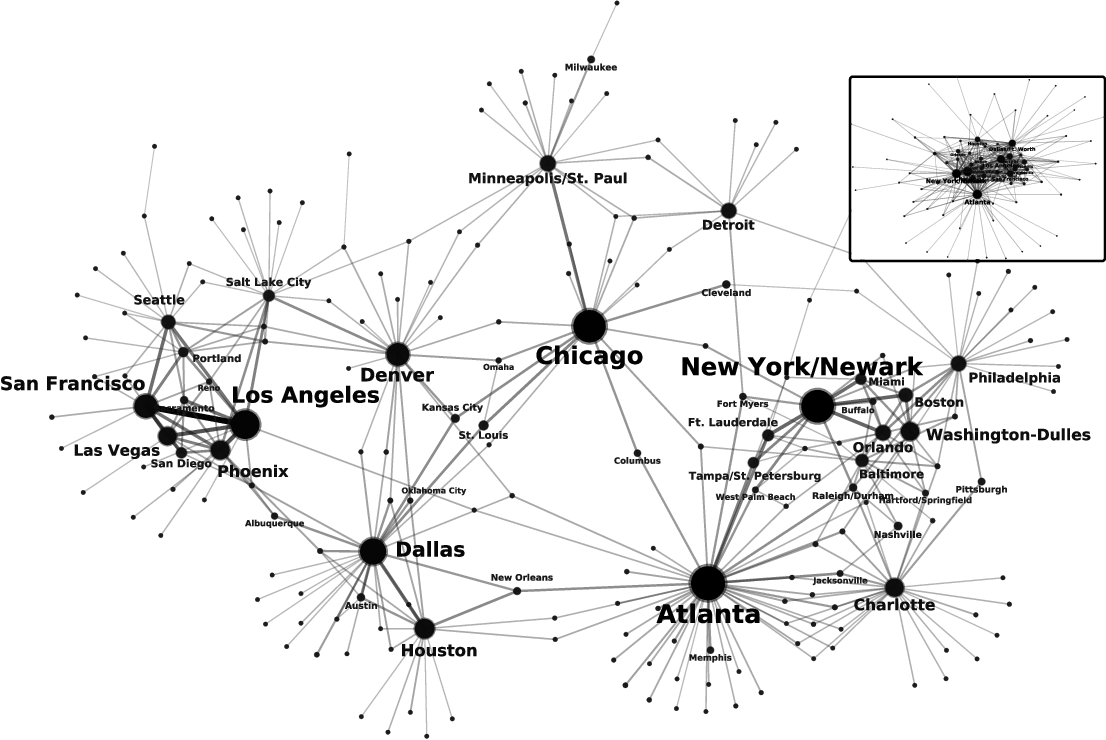
\includegraphics[scale=0.2]{asset/4-Figure2-1.png}
    	\caption{User transportation}
    \end{figure}
  \end{frame}

  \begin{frame}{Social recommendation systems}
  	\vfill
    \begin{itemize}
      \item \textbf{Trust networks}: Groups of related users are considered to have valuable opinion on some matters
      \item \textbf{Improving traditional recommendation systems}
      \item \textbf{Content selection}
    \end{itemize}
    
	\vfill
    \begin{figure}
    	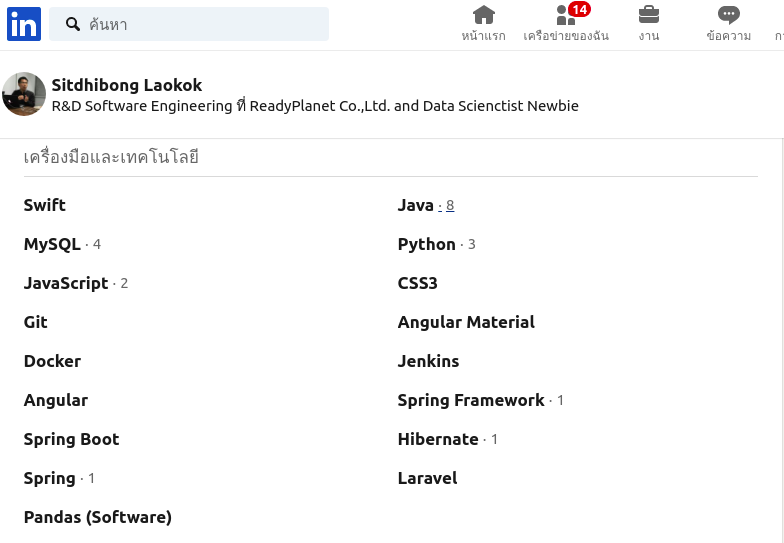
\includegraphics[scale=0.2]{asset/trusted-network.png}
    	\caption{Trust networks}
    \end{figure}
    
  \end{frame}
  
  \section{Social Interaction Analysis}
  \comment{
  \begin{frame}{Cacading}
    \begin{itemize}
      \item \textbf{Properties observed}: \textit{Most cascades have small depth}, \textit{shallow}, \textit{occur in short period}
      \item \textbf{Information origins}:
      \item \textbf{How topology influences cascades}: Topics can reach initially more than one community of users tend to cause larger cascades.
      \item \textbf{Cascades from historical events}: 
    \end{itemize}
  \end{frame}

  \begin{frame}{Prediction cascades}
    \begin{itemize}
      \item<1-> \textbf{Feature selection}: There are 4 main classes of features in generally chosen: \textit{(a) message feature}, \textit{(b) user features}, \textit{(c) network features}, and \textit{(d) temporal features}
      
      \item<2-> \textbf{Message features}: In case of Twitter, Message features can be \textit{# retweet, favorite}, \textit{# hasttags}
      \item<3-> \textbf{User features}: \textit{Connection number (follower and following number)}
      \item<4-> \textbf{Network features}: \textit{Network structure}, \textit{Number of communities involved}
      \item \textbf{Temporal featrues}: \textit{range, speed, power} 
    \end{itemize}
  \end{frame}
  }

  \begin{frame}{Rumors diffusion}
  	
  	\vfill
    \begin{itemize}
      \item \textbf{Characterinzing rumors}: \only<1->{Text's features and the characteristic of users involved in the propagation of the information}
      \item \textbf{Rumor containment rumors}: \only<2>{To detect source of rumors, \textbf{"rumors centrality"} was deveoped}
    \end{itemize}
    
    \vfill
    \begin{figure}
    	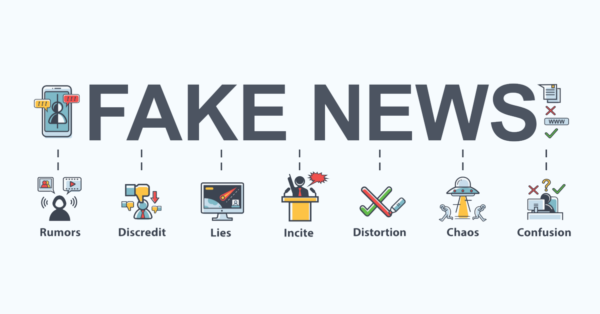
\includegraphics[scale=0.4]{asset/fake-news.png}
    \end{figure}
    
  \end{frame}

  \section{}  
  \begin{frame}
  	\Large{Thank you}
  \end{frame}

\end{document}